\documentclass[12pt]{article}

	
	
	

	%Packages Used%
	\usepackage[utf8]{inputenc}
	\usepackage[round, authoryear]{natbib}
	\usepackage{graphicx}
	\usepackage[USenglish]{babel}
	\usepackage[colorlinks,citecolor=blue,urlcolor=blue,bookmarks=false,hypertexnames=true,linkcolor=black]{hyperref} 
	\usepackage{etoolbox}
	\usepackage{watermark}
	\usepackage{tcolorbox}
	\usepackage[english]{babel}
    \usepackage{graphicx}
    \usepackage[table,xcdraw]{xcolor}
	
	%Packages for flowchart
	\usepackage{amsmath}
    \usepackage{tikz}
    \usepackage{mathdots}
    \usepackage{yhmath}
    \usepackage{cancel}
    \usepackage{color}
    \usepackage{siunitx}
    \usepackage{array}
    \usepackage{multirow}
    \usepackage{amssymb}
    \usepackage{gensymb}
    \usepackage{tabularx}
    \usepackage{booktabs}
    \usepackage{courier}
    \usepackage{tgcursor}
    \usetikzlibrary{fadings}



	
	%Patch it so hyperref only highlights the year in citations
		\makeatletter
	
	% Patch case where name and year are separated by aysep
	\patchcmd{\NAT@citex}
	{\@citea\NAT@hyper@{%
			\NAT@nmfmt{\NAT@nm}%
			\hyper@natlinkbreak{\NAT@aysep\NAT@spacechar}{\@citeb\@extra@b@citeb}%
			\NAT@date}}
	{\@citea\NAT@nmfmt{\NAT@nm}%
		\NAT@aysep\NAT@spacechar\NAT@hyper@{\NAT@date}}{}{}
	
	% Patch case where name and year are separated by opening bracket
	\patchcmd{\NAT@citex}
	{\@citea\NAT@hyper@{%
			\NAT@nmfmt{\NAT@nm}%
			\hyper@natlinkbreak{\NAT@spacechar\NAT@@open\if*#1*\else#1\NAT@spacechar\fi}%
			{\@citeb\@extra@b@citeb}%
			\NAT@date}}
	{\@citea\NAT@nmfmt{\NAT@nm}%
		\NAT@spacechar\NAT@@open\if*#1*\else#1\NAT@spacechar\fi\NAT@hyper@{\NAT@date}}
	{}{}
	
	\makeatother




\begin{document}
    \setcitestyle{authoryear}
	
	


	\author{\textbf{Benjamin Andrea Schüpbach}\\ \\Matr.No. 14-100-564\\benjamin.schuepbach@students.unibe.ch\\Master's Student in Geography\\Institute of Geography, University of Bern\\}
	
	\date{\today}
	
	\title{\textbf{ICARUS\\}}
	\date{\today}
	\maketitle



	\newpage
	
	  

\thispagestyle{empty}



\hspace{0pt}
\vfill
    \begin{center}
        Mein lieber Sohn, fliege nicht zu tief, damit die Federn nicht ins Meerwasser tauchen, sonst werden sie feucht und ziehen dich in die Tiefe. Fliege aber auch nicht zu hoch, sonst schmilzt die Sonne das Wachs, die Flügel fallen auseinander, und du stürtzt ab. Fliege die Mittelstrasse zwischen Meer und Sonne immer nur hinter mir her!
        
        \medbreak
        
        - \textit{Daidalos und Ikaros}, \cite{schwab1990}
    \end{center}
\vfill
\hspace{0pt}

	
	\newpage
	\pagenumbering{roman}
	
	asdfasdf
	
	\newpage
	
	\pagenumbering{arabic}
	\tableofcontents
	
	\newpage
	
		
	\section{Introduction}
	
	Explain how the introduction is structured.
		
		\subsection{Sustainable Development}
    		This section introduces the concept of Sustainable Development (SD). After a brief overview of its origins, some of the many important steps in the adoption of SD into today's global politics by the United Nations are highlighted before various key models are introduced. Finally some of the current measures used to globally advance efforts of SD are presented.
		
		    \subsubsection{Origins of Sustainable Development}
		        Ulrich \citet{grober2007} describes how today's notion of Sustainable Development originated from the concept of Sustainability. Grober further elaborates on how the term "Sustainability" was first introduced to the domain of forestry through Hanns-Carl von Carlowitz \citet{voncarlowitz1732} with his \textit{magnum opus} "Sylvicultura Oeconomica" in which he described the necessity of a controlled and sustained use of timber. Timber was an essential resource at the time, that could not be substituted. According to Grober (\citeyear{grober2007}:18), von Carlowitz criticized "the contemporary short-termed way of thinking which was centred solely on making money", thus emphasizing that society should assure a steady supply of timber through conservation and reforestation efforts in order to guarantee the continual and sustained use of the resource.
		        \medskip
		        
		        The following centuries saw authors like Thomas Robert Malthus (\citeyear{malthus1926}) and George Perkins Marsh (\citeyear{marsh1965}) as well as the Club of Rome (\citeyear{meadows1972a}) publish concerns about human overpopulation, resource shortages and a possible system collapse of the world as it was. In The Limits to growth, Donella Meadows and the Club of Rome (\citeyear{meadows1972a}:23) concluded that "if the present growth trends in world population, industrialization, pollution, food production, and resource depletion continue unchanged, the limits to growth on this planet will be reached sometime within the next one hundred years. The most probable result will be a rather sudden and uncontrollable decline in both population and industrial capacity". Jacobus A. du Pisani (\citeyear{dupisani2006}) gives a comprehensive and detailed overview of this period in the history of the idea of Sustainable Development and the various theories on development and progress that preceded it.
		        \medskip
		        
		        More than 200 years would pass after Carlowitz' concerns until the modern notion of Sustainable Development was introduced formally into global politics. Michael \citet{redclift2005} explains that through the report on global environment and development by the \textit{Brundtland Commission}, or "World Commission on Environment and Development" (\citeyear{wced1987}), the term "Sustainable Development" was introduced into political vocabulary. Gro Harlem Brundtland (\citeyear{brundtland1987}:292),  who headed the commission, defines Sustainable Development as development that meets "[...] the needs and aspirations of the present generation without compromising the ability of future generations to meet their needs".
		        
		        
		    
		    \subsubsection{Sustainable Development as a Geopolitical Paradigm}
		        The Brundtland definition is the cornerstone of Sustainable Development as it is known today. And while it was the Brundtland Report that introduced SD into political agendas arond the world, the need for specific, quantifiable goals to work towards arose \citep{dupisani2006}. Shantayanan Devarajan et al. (\citeyear{devarajan2002}) as well as David Hulme (\citeyear{hulme2009}) illustrate the progression from just the idea of SD, through major stepping-stones like the \textit{United Nations Conference on Environment and Development} in Rio de Janeiro (in 1992), the \textit{International Conference on Population and Development} in Cairo (in 1994) and the \textit{World Summit on Social Development} in Copenhagen (in 1995), to the first major global development framework: the Millennium Development Goals (MDGs).
		        
		        \medskip
		        
		        The MDGs were introduced in September 2000 at the \textit{United Nations Millennium Summit} in New York City (UN General Assembly, \citeyear{ungeneralassembly2000}). These Goals were aimed at issues of poverty, hunger, primary education, gender equality, child mortality, maternal health, preventable diseases, environmental sustainability and a global partnership for development. Towards the end of the 15 year period of the MDGs, Jeffrey David Sachs (\citeyear{sachs2012}:2206) states that "developing countries have made substantial progress towards achievement of the MDGs, although the progress is highly variable across goals, countries, and regions". He further explains how the world has entered a new geological epoch in which human activity has become the most dominant force in fundamental earth dynamics. 
		        
		        \medskip
		        
		        While this notion is not universally accepted, it illustrates a further shift in societal consciousness towards Sustainable Development \citep{heikkurinen2019}. Sachs (\citeyear{sachs2012}:2207) further argues that "in view of [...] dire and unprecedented challenges, the need for urgent, high-profile, and change-producing global goals should be obvious". The MDGs brought sustainability onto the global political main stage and turned Sustainable Development into a geopolitical paradigm. Yet most of the challenges the MDGs were addressing persisted at least to some degree past their expiration date \citep{sachs2012}.
		        

		    \subsubsection{17 Goals to Transform Our World}
	            
	            Because of these persistent challenges, the UN General Assembly adopted the new 2030 Agenda for Sustainable Developments on 25 September 2015 \citep{unitednations2018}. The new agenda consists of 17 goals and originally included 169 subordinate targets, making it the most extensive global development framework to date (UN Statistics Division, \citeyear{unitednationsstatisticsdivision2019a}). Compared to the MDGs, the SDGs thus cover more dimensions of development more specifically (see table X). In March of 2018 as well as one year later in March of 2019, the list of indicators for the SDGs was expanded to 232 total indicators (UN Statistics Division, \citeyear{unitednationsstatisticsdivision2019}). All indicators are classified in tiers that determine their conceptual clarity and progress towards methodological standards for data collection:
	            
	            \medskip
	            
	            \begin{tcolorbox}
    				\textbf{Tier I:} Indicator is conceptually clear, has an internationally established methodology and standards are available, and data are regularly produced by countries for at least 50 per cent of countries and of the population in every region where the indicator is relevant.
    				\medskip
    				
    				\textbf{Tier II:} Indicator is conceptually clear, has an internationally established methodology and standards are available, but data are not regularly produced by countries.
    				\medskip
    				
    				\textbf{Tier III:} No internationally established methodology or standards are yet available for the indicator, but methodology/standards are being (or will be) developed or tested.
    				
    				\begin{center}
    				    (UN Statistics Division, \citeyear{unitednationsstatisticsdivision2019b})
    				\end{center}
			    \end{tcolorbox}

	            \medskip
	            
	            \begin{table}[]
\resizebox{\textwidth}{!}{%
\begin{tabular}{@{}lll@{}}
\toprule
\textbf{Goal} & \textbf{SDGs (2015-2030)}               & \textbf{MDGs (2000-2015)}                   \\ \midrule
1             & No Poverty                              & Eradicate Extreme Poverty and Hunger        \\
2             & Zero Hunger                             & Achieve Universal Primary Education         \\
3             & Good Health and Well-Being              & Promote Gender Equality and Empower Women   \\
4             & Quality Education                       & Reduce Child Mortality                      \\
5             & Gender Equality                         & Improve Maternal Health                     \\
6             & Clean Water and Sanitation              & Combat HIV/AIDS, Malaria and other Diseases \\
7             & Affordable and Clean Energy             & Ensure Environmental Sustainability         \\
8             & Decent Work and Economic Growth         & Global Partnership for Development          \\
9             & Industry, Innovation and Infrastructure &                                             \\
10            & Reduced Inequalities                    &                                             \\
11            & Sustainable Cities and Communities      &                                             \\
12            & Responsible Consumption and Production  &                                             \\
13            & Climate Action                          &                                             \\
14            & Life Below Water                        &                                             \\
15            & Life on Land                            &                                             \\
16            & Peace, Justice and Strong Institutions  &                                             \\
17            & Partnerships                            &                                             \\ \bottomrule
\end{tabular}%
}
\caption{Comparison between SDGs and MDGs.}
\end{table}
	            

	       \subsubsection{The Rural Access Index}
	            
	            The main focus of this thesis is on SDG 9, indicator 1.1: \textit{Proportion of the rural population who live within 2 km of an all-season road} (see chapters X, X and X). Until December 31 of 2018 indicator 9.1.1 was classified as a tier III indicator \citep{sdsn2015}. Today, it is classified as a tier II indicator (UN Statistics Division, \citeyear{unitednationsstatisticsdivision2019b}). The indicator was first introduced by Peter Roberts et al. \citeyear{roberts2006} as the rural access index (RAI) in the context of the Results Measurement System (RMS) of the International Development Association. 
	            
	            \medskip
	            
	             \begin{tcolorbox}
    				
    				"In practice the RAI \textit{measures the number of rural people who live within two kilometers} (typically equivalent to a walk of 20-25 minutes) \textit{of an all-season road as a proportion of the total rural population.} An “all-season road” is a road that is motorable all year round by the prevailing means of rural transport (typically a pick-up or a truck which does not have four-wheel-drive). Occasional interruptions of short duration during inclement weather (e.g. heavy rainfall) are accepted, particularly on lightly trafficked roads."
    				
    				\begin{center}
    				    Roberts et al. (\citeyear{roberts2006}:2)
    				\end{center}
			    \end{tcolorbox}

	            \medskip
                
                According to Roberts et al. (\citeyear{roberts2006}:4), RAI should be measured "by analysis of household surveys that include appropriate questions about access to transport. The aim is to integrate this with the measurement of household characteristics such as income and access to services such as education, health and clean water supply". Although this methodological approach has since been updated, RAI is still considered to be among the most important global development indicators of the transport in the Metadata-Repository of the SDGs (UN Statistics Division, \citeyear{unitednationsstatisticsdivision2019a}). 
                
                \medskip
                
                Today's official methodological approach suggested by the Transport \& ICT Report (\citeyear{transportict2016}) titled \textit{Measuring Rural Access: using new technologies}, uses a combination of geospatial data (more specifically population distribution data, urban extent data, vectorized road data, measurements of road utility status) with a final spatial resolution of 100mx100m as opposed to data from household surveys. The requirements for the calculation of RAI are sturctured into three seperate data requirement domains. It is in the domain of measuring road condition (data requirement 3) where this thesis aims to make a contribution (see section X). Therefore, data requirement 1 (population distribution data) as well as data requirement 2 (urban extent data and vectorized road data) are not introduced further in this section.  
                \medskip
                
                
            \subsubsection{Challenges in Measuring Road Condition}
            
                The following section elaborates on remaining challenges concerning costs, information delay and expenditure of human labour in the Transport \& ICT Report. Table X gives an overview of what the Transport \& ICT Report suggests as suitable sources for road condition data, along with some of their respective advantages and disadvantages.
                
                \medskip
                
                Apart from "Free Apps for Road Assessment", all of the potential data sources are liable to pay costs. The Transport \& ICT Report (\citeyear{transportict2016}:22) states that "it is always possible to collect the necessary condition data with reasonable accuracy, although at a cost". The costs for data collection are directly linked to the availability of data and the processing steps needed to extract relevant information, as well as initial investments for equipment (e.g. high initial investment costs for unmanned aerial drones).
              
                \begin{table}[]{
\small
    \begin{tabular}{p{2.8cm}p{4.6cm}p{4.6cm}}
    
    
    \toprule
    
    \textbf{Data Source} & \textbf{Advantage} & \textbf{Disadvantage} \\ \midrule
   ~&~&~\\
   
   \textbf{Road Inventory Survey} & 
     
      Technically solid,\newline
      consistent with government responsibility
     
     & 
     
      Costsly,
     
     
      Irregular updates,
     
     
      country-specific assessment standards
     
     \\
    \textbf{Satellite \newline Imagery} &
     
      Consistency across \newline countries,
     
     
      potential for high frequency data collection
     
     & 
     
      Costs,
     
      Technically challenging to identify road condition in detail,
     
     
      significant computational process required
     
     \\
    \textbf{Unmanned Aerial Drones} &
     
      Good mobility
     
     & 
     
      Technically challenging,
     
     
      computational \newline process required
     
     \\
    \textbf{Call \newline Detail Record} & 
     
      Consistency across \newline countries,
     
     
      potential for high frequency data collection
     
     & 
     
      Access to data,
     
     
      noise in data
     
     \\
    \textbf{Free Apps \newline for Road Assessment} & 
     
      Cost effective,
     
     
      Potential contribution through crowd-sourcing
     
     &
     
      Statistical errors between measured IRI and actual roughness
     
     \\
    \textbf{Commercial Apps for Road Assessment} & 
     
      Relevant analytical tools provided together
     
     & 
     
      Statistical errors between measured IRI and actual roughness
     
     \\
    \bottomrule
    
    
    
    \end{tabular}}
    \begin{center}
        \caption{Summary of possible sources for road condition data (Transport \& ICT, \citeyear{transportict2016}:23).}
    \end{center}
    

\end{table}
                
                \medskip
                
                In terms of information delay, satellite imagery and unmanned aerial drones offer a lot of flexibility. Meanwhile, data from road inventory surveys, call detail records (georeferenced information about calls made/received, owned by cell phone carriers) and applications for road surface assessment rely on the frequency of surveys, recorded drives or calls made for timeliness. Depending on these factors, data availability may be good or lagging behind.

                
                \medskip
                
                All potential data sources for modern RAI calculation are to some degree labour intensive. International, standardized procedures using satellite imagery, unmanned aerial drones, call detail records or data gathered through mobile applications can reduce initial and upkeep costs, however.
                
                \medskip
                
                
                
                
                
                
                
                \bigskip
	            Dobermann and Nelson 2013: Dobermann, A. and Nelson, R. et al. (2013). Solutions for Sustainable Agriculture and Food Systems. Technical report of the Thematic Group on Sustainable Agriculture and Food Systems. Paris, France and New York, USA: SDSN.
	            
	            \medskip

	            \medskip
	            
		
		
		\subsection{Development Disparities}
		
		
		
		\subsection{Big Data}
			\subsubsection{Big Data Analyses}
			
			\subsubsection{Big Data for Sustainability}
			
			\subsubsection{title}
			
			
			
		\subsection{Image Classification}
			\subsubsection{Deep Neural Networks}
			
			\subsubsection{YOLO \& Darkflow}
			
			\subsubsection{title}
			
			\subsubsection{title}
			
			
			
		\subsection{Goals of this Study}
		
		Show potentials of big data in combination with machine learning for indicators of SDGs.
		
		
		
			\subsubsection{Research Questions}
			
			In this section, research questions based on the goals of this study are formulated. Research questions 1 and 1.1 are directly linked to target indicator 9.1.1 of the SDGs (see section X). Research question 2 is oriented towards the potential overall contribution of Big Data for Sustainability.
			
			\bigskip
			
			\begin{tcolorbox}
				\textbf{Research Question 1:} \smallskip Can georeferenced data for indicator 9.1.1 (RAI) of the SDGs be generated using a Deep Neural Network on the Twitter Streaming API?
			\end{tcolorbox}
			
			\bigskip
				
				\begin{tcolorbox}
					(If answer to RQ1 is yes:) \textbf{Research Question 1.1:} \smallskip Are these data comparable to conventional data for indicator \#58 of the SDGs in terms of quality and accuracy?
				\end{tcolorbox}
				
			\bigskip
				
				\begin{tcolorbox}
					\textbf{Research Question 2:} \smallskip What are potentials and limitations of Big Data analyses for the monitoring of the SDGs?
				\end{tcolorbox}

			\bigskip
				
	
			
	
	\newpage
	
	\section{Methods}
	This section gives an overview of the methods used to conduct this study. It is structured chronologically in the sense of data processing steps (see also figure X). First, the potential data sources are introduced. Second, the process of harvesting the images used to train ICARUS is explained, as well as the methods used to train the algorithm. In the third subsection validation procedures used are shown. The fourth part explains how ICARUS was run. The final section covers how the results form running ICARUS were mapped.
	\bigskip
	
	Explain Flowchart here
	
	\bigskip
	
	\begin{figure}
        \centering
	    


\tikzset{every picture/.style={line width=0.75pt}} %set default line width to 0.75pt        

\begin{tikzpicture}[x=0.75pt,y=0.75pt,yscale=-1,xscale=1]
%uncomment if require: \path (0,660); %set diagram left start at 0, and has height of 660

%Flowchart: Process [id:dp3971687376584736] 
\draw   (199.68,60.33) -- (372.52,60.33) -- (372.52,130.33) -- (199.68,130.33) -- cycle ;
%Straight Lines [id:da3722057941016612] 
\draw    (285.02,130.6) -- (285.02,167.4) ;
\draw [shift={(285.02,169.4)}, rotate = 270] [color={rgb, 255:red, 0; green, 0; blue, 0 }  ][line width=0.75]    (10.93,-3.29) .. controls (6.95,-1.4) and (3.31,-0.3) .. (0,0) .. controls (3.31,0.3) and (6.95,1.4) .. (10.93,3.29)   ;

%Flowchart: Process [id:dp7915450261326966] 
\draw   (199.6,169.33) -- (372.43,169.33) -- (372.43,239.33) -- (199.6,239.33) -- cycle ;
%Flowchart: Process [id:dp31890687546180385] 
\draw   (199.68,280.33) -- (372.52,280.33) -- (372.52,350.33) -- (199.68,350.33) -- cycle ;
%Flowchart: Process [id:dp1798468479163131] 
\draw   (199.1,459.33) -- (371.93,459.33) -- (371.93,529.33) -- (199.1,529.33) -- cycle ;
%Flowchart: Process [id:dp8194881297537675] 
\draw   (199.6,389.79) -- (267.18,389.79) -- (267.18,417.17) -- (199.6,417.17) -- cycle ;
%Flowchart: Process [id:dp5454108064950349] 
\draw   (199.6,570.33) -- (372.43,570.33) -- (372.43,640.33) -- (199.6,640.33) -- cycle ;
%Flowchart: Process [id:dp3149621536877212] 
\draw   (304.85,389.79) -- (372.43,389.79) -- (372.43,417.17) -- (304.85,417.17) -- cycle ;
%Straight Lines [id:da3000291100753305] 
\draw    (285.02,241) -- (285.02,277.4) ;
\draw [shift={(285.02,279.4)}, rotate = 270] [color={rgb, 255:red, 0; green, 0; blue, 0 }  ][line width=0.75]    (10.93,-3.29) .. controls (6.95,-1.4) and (3.31,-0.3) .. (0,0) .. controls (3.31,0.3) and (6.95,1.4) .. (10.93,3.29)   ;

%Straight Lines [id:da3779446467217289] 
\draw    (235.32,416.5) -- (235.51,457.7) ;
\draw [shift={(235.52,459.7)}, rotate = 269.73] [color={rgb, 255:red, 0; green, 0; blue, 0 }  ][line width=0.75]    (10.93,-3.29) .. controls (6.95,-1.4) and (3.31,-0.3) .. (0,0) .. controls (3.31,0.3) and (6.95,1.4) .. (10.93,3.29)   ;

%Straight Lines [id:da5478043110101576] 
\draw    (338.82,416.8) -- (339.01,458) ;
\draw [shift={(339.02,460)}, rotate = 269.73] [color={rgb, 255:red, 0; green, 0; blue, 0 }  ][line width=0.75]    (10.93,-3.29) .. controls (6.95,-1.4) and (3.31,-0.3) .. (0,0) .. controls (3.31,0.3) and (6.95,1.4) .. (10.93,3.29)   ;

%Straight Lines [id:da36668666505152103] 
\draw    (286.02,529.2) -- (286.21,570.4) ;
\draw [shift={(286.22,572.4)}, rotate = 269.73] [color={rgb, 255:red, 0; green, 0; blue, 0 }  ][line width=0.75]    (10.93,-3.29) .. controls (6.95,-1.4) and (3.31,-0.3) .. (0,0) .. controls (3.31,0.3) and (6.95,1.4) .. (10.93,3.29)   ;

%Straight Lines [id:da9485100671630313] 
\draw    (285.02,350.6) -- (236.7,388.17) ;
\draw [shift={(235.12,389.4)}, rotate = 322.13] [color={rgb, 255:red, 0; green, 0; blue, 0 }  ][line width=0.75]    (10.93,-3.29) .. controls (6.95,-1.4) and (3.31,-0.3) .. (0,0) .. controls (3.31,0.3) and (6.95,1.4) .. (10.93,3.29)   ;

%Straight Lines [id:da9817319309154029] 
\draw    (285.02,350.6) -- (337.9,389.02) ;
\draw [shift={(339.52,390.2)}, rotate = 216] [color={rgb, 255:red, 0; green, 0; blue, 0 }  ][line width=0.75]    (10.93,-3.29) .. controls (6.95,-1.4) and (3.31,-0.3) .. (0,0) .. controls (3.31,0.3) and (6.95,1.4) .. (10.93,3.29)   ;

%Flowchart: Process [id:dp8914422903741139] 
\draw  [color={rgb, 255:red, 74; green, 74; blue, 74 }  ,draw opacity=0.8 ] (442.77,169.33) -- (574.02,169.33) -- (574.02,239.33) -- (442.77,239.33) -- cycle ;
%Flowchart: Process [id:dp3094514982649226] 
\draw  [color={rgb, 255:red, 74; green, 74; blue, 74 }  ,draw opacity=0.8 ] (442.77,279.4) -- (574.02,279.4) -- (574.02,349.4) -- (442.77,349.4) -- cycle ;
%Flowchart: Process [id:dp6350575730299324] 
\draw  [color={rgb, 255:red, 74; green, 74; blue, 74 }  ,draw opacity=0.8 ] (442.77,459.33) -- (574.02,459.33) -- (574.02,529.33) -- (442.77,529.33) -- cycle ;
%Flowchart: Process [id:dp4180968434721368] 
\draw  [color={rgb, 255:red, 74; green, 74; blue, 74 }  ,draw opacity=0.8 ] (442.77,370) -- (574.02,370) -- (574.02,440) -- (442.77,440) -- cycle ;
%Straight Lines [id:da5306027300225034] 
\draw [color={rgb, 255:red, 74; green, 74; blue, 74 }  ,draw opacity=0.8 ]   (371.93,315.1) -- (440.77,315.49) ;
\draw [shift={(442.77,315.5)}, rotate = 180.32] [color={rgb, 255:red, 74; green, 74; blue, 74 }  ,draw opacity=0.8 ][line width=0.75]    (10.93,-3.29) .. controls (6.95,-1.4) and (3.31,-0.3) .. (0,0) .. controls (3.31,0.3) and (6.95,1.4) .. (10.93,3.29)   ;

%Straight Lines [id:da6129943654827146] 
\draw [color={rgb, 255:red, 74; green, 74; blue, 74 }  ,draw opacity=0.8 ]   (371.93,205.1) -- (440.77,205.49) ;
\draw [shift={(442.77,205.5)}, rotate = 180.32] [color={rgb, 255:red, 74; green, 74; blue, 74 }  ,draw opacity=0.8 ][line width=0.75]    (10.93,-3.29) .. controls (6.95,-1.4) and (3.31,-0.3) .. (0,0) .. controls (3.31,0.3) and (6.95,1.4) .. (10.93,3.29)   ;

%Straight Lines [id:da06735980977616274] 
\draw [color={rgb, 255:red, 74; green, 74; blue, 74 }  ,draw opacity=0.8 ]   (371.93,404.7) -- (440.77,405.09) ;
\draw [shift={(442.77,405.1)}, rotate = 180.32] [color={rgb, 255:red, 74; green, 74; blue, 74 }  ,draw opacity=0.8 ][line width=0.75]    (10.93,-3.29) .. controls (6.95,-1.4) and (3.31,-0.3) .. (0,0) .. controls (3.31,0.3) and (6.95,1.4) .. (10.93,3.29)   ;

%Straight Lines [id:da1328641994921984] 
\draw [color={rgb, 255:red, 74; green, 74; blue, 74 }  ,draw opacity=0.8 ]   (371.93,495.1) -- (440.77,495.49) ;
\draw [shift={(442.77,495.5)}, rotate = 180.32] [color={rgb, 255:red, 74; green, 74; blue, 74 }  ,draw opacity=0.8 ][line width=0.75]    (10.93,-3.29) .. controls (6.95,-1.4) and (3.31,-0.3) .. (0,0) .. controls (3.31,0.3) and (6.95,1.4) .. (10.93,3.29)   ;


% Text Node
\draw (286.1,95.33) node  [align=left] {{\fontfamily{pcr}\selectfont TWITTER API}};
% Text Node
\draw (372.43,149.8) node [scale=0.9,color={rgb, 255:red, 74; green, 74; blue, 74 }  ,opacity=1 ] [align=left] {{\fontfamily{pcr}\selectfont {\small FILTER: GEO/MEDIA}}};
% Text Node
\draw (371.43,260) node [scale=0.9,color={rgb, 255:red, 74; green, 74; blue, 74 }  ,opacity=1 ] [align=left] {{\fontfamily{pcr}\selectfont {\small PASS THROUGH}}};
% Text Node
\draw (371.43,372) node [scale=0.9,color={rgb, 255:red, 74; green, 74; blue, 74 }  ,opacity=1 ] [align=left] {{\fontfamily{pcr}\selectfont {\small DETECTION?}}};
% Text Node
\draw (371.43,551.8) node [scale=0.9,color={rgb, 255:red, 74; green, 74; blue, 74 }  ,opacity=1 ] [align=left] {{\fontfamily{pcr}\selectfont {\small CARTOPY}}};
% Text Node
\draw (286.02,204.33) node  [align=left] {{\fontfamily{pcr}\selectfont RAW DATA}};
% Text Node
\draw (286.1,315.33) node  [align=left] {{\fontfamily{pcr}\selectfont ICARUS}};
% Text Node
\draw (286.52,494.33) node  [align=left] {{\fontfamily{pcr}\selectfont SAVE (CSV)}};
% Text Node
\draw (233.39,403.48) node  [align=left] {{\fontfamily{pcr}\selectfont YES}};
% Text Node
\draw (338.64,403.48) node  [align=left] {{\fontfamily{pcr}\selectfont NO}};
% Text Node
\draw (285.02,605.33) node  [align=left] {{\fontfamily{pcr}\selectfont VISUALIZE}};
% Text Node
\draw (508.39,204.33) node [scale=0.8,color={rgb, 255:red, 74; green, 74; blue, 74 }  ,opacity=1 ] [align=left] {{\footnotesize {\fontfamily{ptm}\selectfont Coordinates: lat/lon}}\\{\footnotesize {\fontfamily{ptm}\selectfont Media URL}}\\{\footnotesize {\fontfamily{ptm}\selectfont Datetime}}\\{\footnotesize {\fontfamily{ptm}\selectfont Unique ID}}};
% Text Node
\draw (508.39,314.4) node [scale=0.8,color={rgb, 255:red, 74; green, 74; blue, 74 }  ,opacity=1 ] [align=left] {{\footnotesize {\fontfamily{ptm}\selectfont Image Classifier}}\\{\footnotesize {\fontfamily{ptm}\selectfont (tinyYOLO)}}};
% Text Node
\draw (508.39,405) node [scale=0.8,color={rgb, 255:red, 74; green, 74; blue, 74 }  ,opacity=1 ] [align=left] {{\fontfamily{ptm}\selectfont {\footnotesize Assessment based}}\\{\fontfamily{ptm}\selectfont {\footnotesize on Detection }}\\{\fontfamily{ptm}\selectfont {\footnotesize Threshold}}};
% Text Node
\draw (508.39,494.33) node [scale=0.8,color={rgb, 255:red, 74; green, 74; blue, 74 }  ,opacity=1 ] [align=left] {{\fontfamily{ptm}\selectfont {\footnotesize Coordinates: lat/lon}}\\{\fontfamily{ptm}\selectfont {\footnotesize Media URL}}\\{\fontfamily{ptm}\selectfont {\footnotesize Datetime}}\\{\fontfamily{ptm}\selectfont {\footnotesize ICARUS Predictions}}};


\end{tikzpicture}

	    \caption{Flowchart of Methodology.}
	\end{figure}

	\bigskip
	
	\newpage
	    
	    \subsection{Data Source(s)}
		\subsection{Harvesting of Training Images}
		\subsection{Supervised Classification & Training of ICARUS}
		\subsection{Validation}
		    \subsubsection{Mean Average Precision}
		    \subsubsection{Validation with Google Streetview}
		\subsection{Running ICARUS}
		    \subsubsection{Gathering Actual Data}
		    \subsubsection{Processing with ICARUS}
		\subsubsection{Visualization}

	
	\newpage
	
	\section{Results}
		\begin{figure}[h]
			\centering
			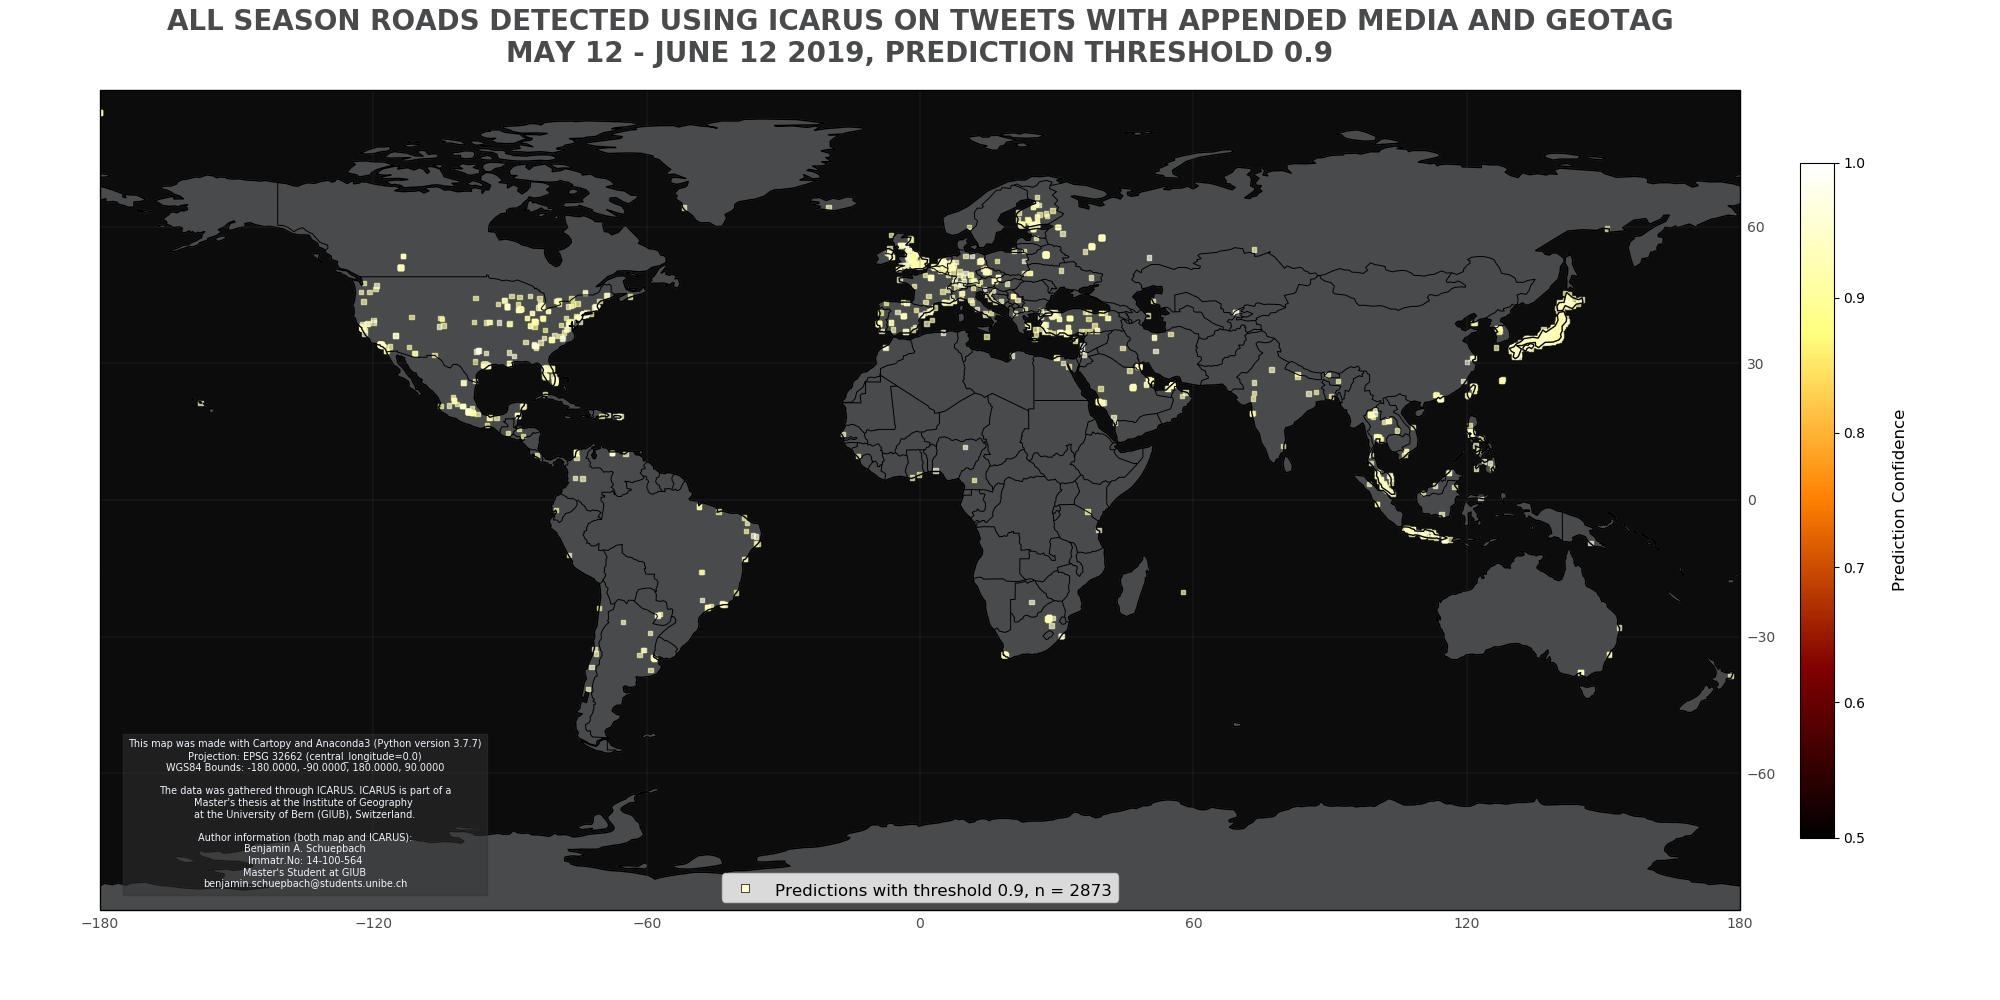
\includegraphics[scale=0.3]{images/map_ICARUS_thresh90}
			\caption{Map of Tweets where ICARUS identified AllSeasonRoads}
		\end{figure}
	
	\newpage

		\section{Discussion}
	
	\subsubsection{Relevance \& Shortcomings}
	\subsubsection{Importance to Sustainable Development}
	

	\newpage
	
		\section{Conclusion \& Outlook}
		\subsubsection{title}

	\newpage

	ADD \{ \} TO BIBLIOGRAPHY ENTRIES THAT AREN'T DISPLAYED CORRECTLY IN THE .BIB FILE
	\bibliographystyle{apa}
	\bibliography{ma_bib}
	

\end{document}